%Input preamble
%Style
\documentclass[12pt]{article}
\usepackage[top=1in, bottom=1in, left=1in, right=1in]{geometry}
\parindent 22pt
\usepackage{fancyhdr}

%Packages
\usepackage{adjustbox}
\usepackage{amsmath}
\usepackage{amsfonts}
\usepackage{amssymb}
\usepackage{bm}
\usepackage[table]{xcolor}
\usepackage{tabu}
\usepackage{color,soul}
\usepackage{makecell}
\usepackage{longtable}
\usepackage{multirow}
\usepackage[normalem]{ulem}
\usepackage{etoolbox}
\usepackage{graphicx}
\usepackage{tabularx}
\usepackage{ragged2e}
\usepackage{booktabs}
\usepackage{caption}
\usepackage{fixltx2e}
\usepackage[para, flushleft]{threeparttablex}
\usepackage[capposition=top,objectset=centering]{floatrow}
\usepackage{subcaption}
\usepackage{pdfpages}
\usepackage{pdflscape}
\usepackage{natbib}
\usepackage{bibunits}
\definecolor{maroon}{HTML}{990012}
\usepackage[colorlinks=true,linkcolor=maroon,citecolor=maroon,urlcolor=maroon,anchorcolor=maroon]{hyperref}
\usepackage{marvosym}
\usepackage{makeidx}
\usepackage{tikz}
\usetikzlibrary{shapes}
\usepackage{setspace}
\usepackage{enumerate}
\usepackage{rotating}
\usepackage{tocloft}
\usepackage{epstopdf}
\usepackage[titletoc]{appendix}
\usepackage{framed}
\usepackage{comment}
\usepackage{xr}
\usepackage{titlesec}
\usepackage{footnote}
\usepackage{longtable}
\newlength{\tablewidth}
\setlength{\tablewidth}{9.3in}
\setcounter{secnumdepth}{4}

\titleformat{\paragraph}
{\normalfont\normalsize\bfseries}{\theparagraph}{1em}{}
\titlespacing*{\paragraph}
{0pt}{3.25ex plus 1ex minus .2ex}{1.5ex plus .2ex}
\makeatletter
\pretocmd\start@align
{%
  \let\everycr\CT@everycr
  \CT@start
}{}{}
\apptocmd{\endalign}{\CT@end}{}{}
\makeatother
%Watermark
\usepackage[printwatermark]{xwatermark}
\usepackage{lipsum}
\definecolor{lightgray}{RGB}{220,220,220}
%\newwatermark[allpages,color=lightgray,angle=45,scale=3,xpos=0,ypos=0]{Preliminary Draft}

%Further subsection level
\usepackage{titlesec}
\setcounter{secnumdepth}{4}
\titleformat{\paragraph}
{\normalfont\normalsize\bfseries}{\theparagraph}{1em}{}
\titlespacing*{\paragraph}
{0pt}{3.25ex plus 1ex minus .2ex}{1.5ex plus .2ex}

\setcounter{secnumdepth}{5}
\titleformat{\subparagraph}
{\normalfont\normalsize\bfseries}{\thesubparagraph}{1em}{}
\titlespacing*{\subparagraph}
{0pt}{3.25ex plus 1ex minus .2ex}{1.5ex plus .2ex}

%Functions
\DeclareMathOperator{\cov}{Cov}
\DeclareMathOperator{\corr}{Corr}
\DeclareMathOperator{\var}{Var}
\DeclareMathOperator{\plim}{plim}
\DeclareMathOperator*{\argmin}{arg\,min}
\DeclareMathOperator*{\argmax}{arg\,max}

%Math Environments
\newtheorem{theorem}{Theorem}
\newtheorem{claim}{Claim}
\newtheorem{condition}{Condition}
\renewcommand\thecondition{C--\arabic{condition}}
\newtheorem{algorithm}{Algorithm}
\newtheorem{assumption}{Assumption}
\renewcommand\theassumption{A--\arabic{assumption}}
\newtheorem{remark}{Remark}
\renewcommand\theremark{R--\arabic{remark}}
\newtheorem{definition}[theorem]{Definition}
\newtheorem{hypothesis}[theorem]{Hypothesis}
\newtheorem{property}[theorem]{Property}
\newtheorem{example}[theorem]{Example}
\newtheorem{result}[theorem]{Result}
\newenvironment{proof}{\textbf{Proof:}}{$\bullet$}

%Commands
\newcommand\independent{\protect\mathpalette{\protect\independenT}{\perp}}
\def\independenT#1#2{\mathrel{\rlap{$#1#2$}\mkern2mu{#1#2}}}
\newcommand{\overbar}[1]{\mkern 1.5mu\overline{\mkern-1.5mu#1\mkern-1.5mu}\mkern 1.5mu}
\newcommand{\equald}{\ensuremath{\overset{d}{=}}}
\captionsetup[table]{skip=10pt}
%\makeindex

\setlength\parindent{20pt}
\setlength{\parskip}{0pt}

\newcolumntype{L}[1]{>{\raggedright\let\newline\\\arraybackslash\hspace{0pt}}m{#1}}
\newcolumntype{C}[1]{>{\centering\let\newline\\\arraybackslash\hspace{0pt}}m{#1}}
\newcolumntype{R}[1]{>{\raggedleft\let\newline\\\arraybackslash\hspace{0pt}}m{#1}}



%Logo
%\AddToShipoutPictureBG{%
%  \AtPageUpperLeft{\raisebox{-\height}{
\includegraphics[width=1.5cm]{uchicago.png}}}
%}

\newcolumntype{L}[1]{>{\raggedright\let\newline\\\arraybackslash\hspace{0pt}}m{#1}}
\newcolumntype{C}[1]{>{\centering\let\newline\\\arraybackslash\hspace{0pt}}m{#1}}
\newcolumntype{R}[1]{>{\raggedleft\let\newline\\\arraybackslash\hspace{0pt}}m{#1}}

\newcommand{\mr}{\multirow}
\newcommand{\mc}{\multicolumn}

%\newcommand{\comment}[1]{}


\begin{document}

\noindent This section of the appendix assesses some of the critiques to ABC, which could apply to CARE as well. The critiques focus on the first phase of the program, to which we refer simply as ABC in this section of the appendix.\\

\noindent The first critique we assess is that of \citet{}. The author asks if ABC prevented socio-cultural mental retardation. He focuses on different measures of cognition, and generically calls them IQ. His main focus is on the raw mean difference between the treatment and the control groups in the Bayley Mental Development Index (MDI) at age 1.\footnote{The Bayley Mental Development Index is a standard measure of cognition at taken between ages 0 and 2 \citep{•}.} He finds a noticeable difference in the mean difference between cohorts 1 and 2 and cohorts 2 and 4, as early as six months after the treatment began. As \citet{} argues, this difference is conspicuous and we display it in Table~\ref{table:cohorts}. Importantly, the author fails to note that the mean differences have noticeably high standard errors.

\begin{table}[H] 
\begin{threeparttable}
\caption{Treatment - Control Mean Difference by Cohort, ABC}
\label{table:cohorts}
\centering 
\begin{tabular}{lcc} \toprule
 & (1) & (2) \\
 & Bayley MDI, 12 Months & Bayley MDI, 24 Months \\ \midrule
 &  &  \\\
Cohort 1 & 4.841 & -2.901 \\
 & (6.013) & (5.926) \\
Cohort 2 & 0.071 & 1.882 \\
 & (6.013) & (5.830) \\
Cohort 3 & 9.143 & 10.038 \\
 & (5.801) & (5.926) \\
Cohort 4 & 7.829 & 13.713 \\
 & (5.801) & (5.830) \\ \\ \midrule
Observations & 112 & 110 \\
$R^2$ & 0.055 & 0.110 \\ \bottomrule
 \end{tabular}
\begin{tablenotes}
\footnotesize
\item Note: This table displays the mean difference between the treatment and control groups in two measures of the Bayley Mental Development Index, for ABC. Homoskedastic, asymptotic standard errors are in parentheses.
\end{tablenotes}
\end{threeparttable}
\end{table}

\noindent \citet{} states that: ``an essential question is whether the differences at 6 months of age were due to the intervention or where preexisting'' \citep[][p. 230]{•}. \citet{} proceeds with speculative exercises that lead him to state that it is questionable to conclude that the mean difference between the treatment and control groups as early as age six months is a consequence of the treatment.\footnote{The exact quote is: ``Even if the differences between experimental and control groups at 6 months of age were a consequence of the first few months of intervention, which is questionable, the negligible additional effects after age 4.5 more years in the program should at least make one cautious about this kind of intervention's potential [\ldots]'' \citep[][p. 235]{•}. We asses the former point before getting to the latter.}\\

\noindent His argument oscillates from not receiving information on the maternal characteristics which he considers fundamental for his analysis to comparing test scores over the years.\footnote{He does not note that tests scores \textit{do not have a well-defined scale} and are hard to compare.}\\ 

\noindent We make three annotations with respect to the comments in \citet{}.\\ 

\noindent \textbf{1. Neither in cohort 3 nor in cohort 4 do mothers differ in observed characteristics between the treatment and the control groups.} When jointly testing the hypothesis of differences in a battery of observed characteristics, we fail to reject any difference between the families of these children (see Table~\ref{tab:baseline_coh3} and Table~\ref{tab:baseline_coh4}). Even when the point estimates present some differences, they are minimal. For example, treatment-group mothers differ from control-group mothers, on average, by having one more point in the IQ score, which has a population standard deviation of 15.\\

\noindent \textbf{2. Other early childhood education programs have generated gains in cognition very early in life, as soon as after a year of the program's beginning.} A more recent program, the Infant Health and Development Program (IHDP), treated children from ages 0 to 3. \citet{Gross_Spiker_etal_1997_BOOKHelpinglowbirth} thoroughly describe this program. A lot of its elements were based on ABC and CARE. The program offered an average of eight hours a week of center-based childcare from ages 1 to 3, weekly home visits from ages 0 to 1, and bi-monthly home visits from ages 1 to 3. Measures on the Bayley MDI at 12 and 24 months are available. The most intensive part of the treatment, center-based childcare, began at age 12 months in IHDP while it began at birth in ABC. As in ABC, after a few months of center-based childcare, the effects on cognition were substantial in IHDP.
\begin{table}[H] 
\begin{threeparttable}
\caption{Treatment - Control Mean Difference, IHDP}
\label{table:ihdp}
\centering 
\begin{tabular}{lcc} \hline \hline
 & (1) & (2) \\
 & Bayley MDI, 12 Months & Bayley MDI, 24 Months \\ \hline
 &  &  \\\
Mean Treatment - Mean Control & 0.142 & 9.958 \\
 & (0.968) & (1.498) \\
 &  &  \\ \hline
Observations & 893 & 910 \\
$R^2$ & 0.000 & 0.067 \\ \hline \hline  
\end{tabular}
\begin{tablenotes}
\footnotesize
\item Note: This table displays the mean difference between the treatment and control groups in two measures of the Bayley Mental Development Index, for the Infant Health and Development Program using the principal analysis sample. Robust standard errors clustered by state and an indicator of weight below 2,000 grams in parentheses.
\end{tablenotes}
\end{threeparttable}
\end{table}


\noindent \textbf{3. The effects on cognition are sustained throughout childhood and up to age 21 even when partialing out the Bayley MDI at ages 12 and 24 months.} When partialing out in a linear regression the score in the Bayley MDI tests both at twelve and twenty-four months of age, the treatment effects on cognition, measured by the mean difference between the treatment and the control groups in different IQ test scores, are still significant and are sustained up to age 21 (see Figure~\ref{fig:treatiqsabc}).

\begin{figure}[H]
		\caption{Treatment Effects on IQ, ABC} \label{fig:treatiqsabc}
		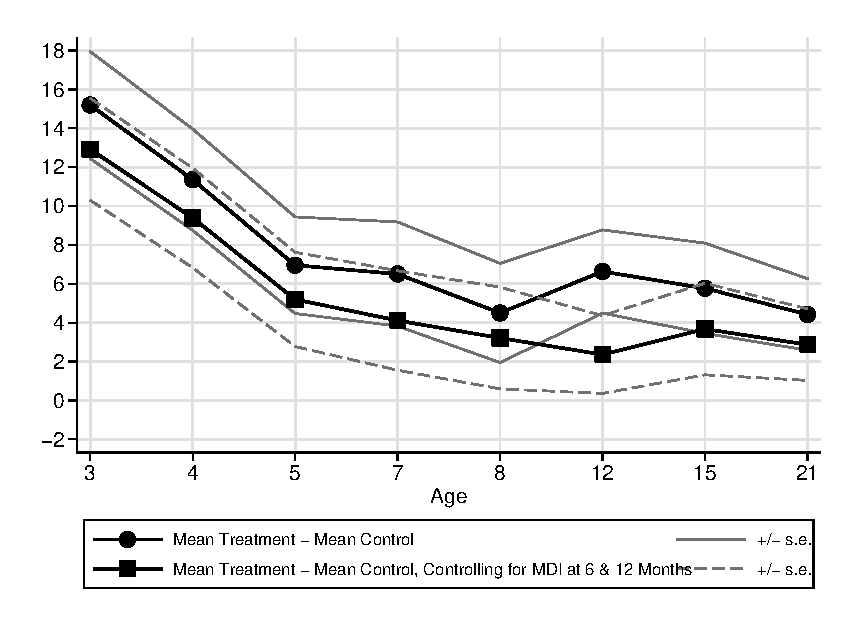
\includegraphics[width=.9\columnwidth]{output/abc_mdifixing_2.eps}
\floatfoot{
\footnotesize
\noindent Note: This figure displays the mean difference between the treatment and the control groups in IQ at different ages, pooling males ans females. The dotted line represents the raw difference. The squared line represents the difference when linearly controlling for the Bayley Mental Development Index at 6 and 12 months.}
\end{figure}

\noindent The author raises an additional concern. He states that even if the early-life effects on the Bayley MDI were true, the effects were not long-lasting. When doing so, he exclusively refers to the effects the program had on cognition. As we vastly document throughout the main paper, however, ABC had effects on a wide set of life-cycle outcomes, which perhaps are more important than the effects on cognition if measures by the economic gains they generate. Examples include: employment at age 30 for males, high-school graduation for females, and a variety of health measures at age 34 for males. We document these effects in the main paper.\\

\noindent This critique relates to a second critique that has been made to ABC. Mostly based on the fade-out of the effects on cognition and on results on age-21 outcomes, some studies claim that ABC had no sustained long-term effects. In addition to the evidence we cite above, it is important to add the following. \textbf{4. The treatment effects of ABC differed by gender.} For example, we find substantial effects on employment for males and high-school graduation for females. This does not mean that the program did not work. It means that market conditions could affect the way in which the participants of the program could have benefited from its effects.\\

\newgeometry{top=.5in, bottom=.5in, left=.5in, right=.5in}

\begin{sidewaystable}[H] 
\begin{threeparttable}
\caption{Randomization Compromises, ABC and CARE}
\label{table:compromised}
\centering
\tiny
\begin{tabular}{cccccc} \hline \hline
Case & Child ID & Initial Assignment & Compromise Description & Data Availability & Methodology Assumption \\ \\ \hline
\multicolumn{6}{l}{\textbf{ABC}} \\ 
1 & N/A (Case A) & Treatment & Left the study & No data & Missing at random \\
2 & N/A (Case B) & Treatment & Left the study & No data & Missing at random \\
3 & N/A (Case C) & Treatment & Left the study & No data & Missing at random \\
4 & N/A (Case D)          & Treatment & Left the study & No data & Missing at random \\
5 & .x & Control            & Died at age 0, heart disease & Baseline characteristics, any data collection before dead      & Attrition after dead \\
6 & 914 & Control         & Died at age 0, heart disease & Baseline characteristics, any data collection before dead   & Attrition after dead \\
7 & 74 & Treatment      & Died at age 0, SIDS  5 & Baseline characteristics, any data collection before dead & Attrition after dead \\
8 & 99 & Treatment      & Died at age 4, pedestrian accident & Baseline characteristics, any data collection before dead & Attrition after dead \\
9 & 95   & Treatment       & Diagnosed as developmentally delayed at 6 months old   & No data after diagnosis & Dropped from the sample (non-eligible) \\ 
10 & 124 & Treatment       & Diagnosed as developmentally delayed at 36 months old & No data after diagnosis & Dropped from the sample (non-eligible) \\ 
11   & 900 & Treatment  & Did not comply to treatment status  & Baseline characteristics, any data collection up to age 8 & Attrition after age 8  \\
12 & 912 & Treatment  & Did not comply to treatment status  & Baseline characteristics, any data collection up to age 8 & Attrition after age 8 \\
13 & 922 & Treatment  & Did not comply to treatment status  & Baseline characteristics, any data collection up to age 8 & Attrition after age 8 \\
14 & 906 & Treatment  & Abandoned study at 54 months old  & Baseline characteristics, any data collection up to age 54 months & Attrition after age 54 months \\
15 & 82 & Control       & Moved to unspecified place after age 15 &   Baseline characteristics, any data collection up to age 15 & Attrition beginning at age 21 \\
16 &  78  & Control       & Crossover from control to treatment  & Baseline characteristics, any data collection up to age 8 months & Attrition after age 8 \\
17 &  82 & Control       & Crossover from control to treatment due to special needs & Baseline characteristics, any data collection up to age 8 & Dropped from the sample \\ 
18 & 119 & Control       & Crossover from control to treatment due to special needs & Baseline characteristics, any data collection up to age 8 & Dropped from the sample \\ 
19 & 85 & Treatment         & Only 3 months of treatment  & All post-age 21 follow-ups available   & Same as complying treatment children  \\ 
20 & 103 & Treatment         & Only 10 months of treatment  & All post-age 21 follow-ups available   & Same as complying treatment children  \\ 
21 & 108 & Treatment         & Only 6 months of treatment  & All post-age 21 follow-ups available   & Same as complying treatment children  \\ 
22 & 123 & Treatment         & Only 9 months of treatment  & All post-age 21 follow-ups available   & Same as complying treatment children  \\ \\ \hline
\multicolumn{6}{l}{\textbf{CARE}} \\
1 & 310 & Family education & Died at age 0, unknown causes & Baseline characteristics & Attrition after dead \\
2 & 301 & Center-based Childcare  & Abandoned study at age 5  & Baseline characteristics, any data collection up to age 5 & Attrition after age 5 \\
3 & 910 & Control & Move to unspecified place at 11 months old & Baseline characteristics, any data collection up to 11 months old & Attrition beginning at 11 months old interview \\
4 & 142 & Center-based Childcare & Move to unspecified place after age 5 months old & Baseline characteristics, any data collection up to 5 months old & Attrition beginning at 5 months old \\
 &  & and Family Education &  &  & \\
5 & 150 & Center-based Childcare & Move to unspecified place after age 5 & Baseline characteristics, any data collection up to 5 & Attrition beginning at 5 \\
 &  & and Family Education &  &  & \\ \hline \hline 
\end{tabular}
\end{threeparttable}
\end{sidewaystable}

\restoregeometry

\noindent The third and last critique we assess is that of compromised randomization. The main critique to the program with this respect is that seven children in the treatment group did not comply to their initial assignment and one child switched from control to treatment status. This critique refers to the children labeled with the following IDs by the program: N/A Case A, N/A Case B, N/A Case C, N/A Case D, 900, 912, 922, and 78 (see Table~\ref{table:compromised}). Although we document more cases of compromised randomization, we start by assessing these eight cases.\footnote{Our methodology assess all the cases except the children for whom we do not have data at all (Case A, N/A Case B, N/A Case C, N/A Case D). We are not able to account for them because our method is based on observing at least some baseline characteristics. See Section~\ref{section:methodology} in the main paper for more details.}\\

\noindent First, we propose a method to assess the non-compliance of children 900, 912, 922, and 78, for whom we have data available from ages 0 to 8. This allows for the possibility to adjust the mean difference between the treatment and the control groups, using a standard Bloom estimator \citep{Bloom_1984_ER}. This estimator accounts for compliance, by weighting the mean difference by a measure of the probability of compliance. It takes the following form: 

\begin{equation}
\Delta^{\textbf{Bloom}} = \frac{\mathbb{E} \left[ Y | R = 1 \right] - \mathbb{E} \left[ Y | R = 0 \right] }{\mathbb{E} \left[ D = 1 | R = 1 \right] - \mathbb{E} \left[ D = 0 | R = 0 \right]}, 
\end{equation}

\noindent where $R$ indicates randomization into treatment, $D$ indicates treatment take-up, and $Y$ is an outcome of interest.\\

\noindent This estimator has gained attention as it coincides with the instrumental variables estimator of the parameter in linear regression of an outcome on a single explanatory variable, e.g. treatment take-up. As \citet{Angrist_Imbens_ea_1996_JASA} show, under certain assumptions it can be interpreted as the average treatment effect for those individuals induced to take up treatment by the instrument. These interpretation has various weaknesses \citep{Heckman_Urzua_2010_JoE,Heckman_Urzua_etal_2006_REStat}.\\

\noindent To compare the mean difference and the Bloom estimator we consider two measures of cognition, which are commonly used when evaluating ABC and are available for children 900, 912, 922, and 78: the Stanford Binet IQ test at age 3 and the Wechsler Preschool and Primary Scale of Intelligence. Table~\ref{table:ivbloom1} presents the results and shows that the differences are minimal. \textbf{5. Adjusting for the non-compliance of children 900, 912, 922, and 78 makes little difference} when assessing outcomes for which we observe these children. 

\begin{table}[H] 
\begin{threeparttable}
\caption{Assessing Non-compliance in ABC, Exercise 1}
\label{table:nc1}
\centering 
\begin{tabular}{ccccc} \toprule
 & (1) & (2) & (3) & (4) \\
 & IQ, Age 3 & IQ, Age 3  & IQ, Age 5 & IQ, Age 5 \\ \midrule
 &  &  & & \\\
Treatment - Control Mean Difference & 14.970 &  & 6.398 &  \\
 & (2.794) &  & (2.494) &  \\
Bloom &  & 16.245 &  & 6.943 \\
 &  & (2.877) &  & (2.643) \\ \midrule
Observations & 100 & 100 & 100 & 100  \\
 $R^2$ & 0.227 & 0.289 & 0.063 & 0.088 \\ \bottomrule
 \end{tabular}
\begin{tablenotes}
\footnotesize
\item Note: This table displays the mean difference between the treatment and control groups and the same difference adjusted for non-compliance (Bloom estimator) in two measures of IQ, the Stanford-Binet IQ Score at age 3 and the Wechsler Preschool and Primary Scale of Intelligence at age 5. Homoskedastic, asymptotic standard errors are in parentheses.
\end{tablenotes}
\end{threeparttable}
\end{table}


\noindent Second, we propose a method to account for non-compliance of the children N/A Case A, N/A Case B, N/A Case C, N/A Case D. For them, we have no data at all. We reproduce the estimates in Table~\ref{table:nc2}, assigning to each of these four children the worst score across all the children in the treatment group, for each of the tests we consider---the worst score was 71 for both the age-3 and the age-5 measures. \textbf{6. Even when assigning the worst score to the children who did not comply to treatment and for whom no data is available, the mean difference between treatment and control is sizable and not significantly different from the baseline cases where we do not adjust for non-compliance cases} (columns (1) and (3) in Table~\ref{table:nc1}).

\documentclass[]{article}
\setlength{\pdfpagewidth}{8.5in} \setlength{\pdfpageheight}{11in}
\begin{document}
\begin{tabular}{lcccc} \hline
 & (1) & (2) & (3) & (4) \\
 & iq3y\_itt & iq3y\_iv & iq5y\_itt & iq5y\_iv \\
VARIABLES & IQ at age 3y months & IQ at age 3y months & IQ at age 5y months & IQ at age 5y months \\ \hline
 &  &  &  &  \\
Randomization into center-based care (ABC and CARE) & 12.908*** &  & 4.284 &  \\
 & (2.901) &  & (2.647) &  \\
Indicator for the actual treatment receipt for center-based care &  & 15.111*** &  & 5.016* \\
 &  & (3.061) &  & (2.960) \\
 &  &  &  &  \\
Observations & 104 & 104 & 104 & 104 \\
 R-squared & 0.163 & 0.306 & 0.025 & 0.093 \\ \hline
\end{tabular}
\end{document}


\noindent Finally, we note that our methodology in Section~\ref{section:methodology} and the results we present in Section~\ref{section:results} account for the reminder of randomization compromises, as when the families moved or abandoned the study later in the study. \textbf{7. The results are not greatly sensitive to adjusting for the rest of randomization compromises}, as we show in Section~\ref{section:results}.

\end{document} 